\documentclass{article}

\usepackage{fullpage}
\usepackage{color}
\usepackage{amsmath}
\usepackage{url}
\usepackage{verbatim}
\usepackage{graphicx}
\usepackage{parskip}
\usepackage{amssymb}
\usepackage{nicefrac}
\usepackage{listings}

% Answers
\def\ans#1{\par\gre{Answer: #1}}
%\def\ans#1{} % Comment this line to produce document with answers

% Colors
\definecolor{blu}{rgb}{0,0,1}
\def\blu#1{{\color{blu}#1}}
\definecolor{gre}{rgb}{0,.5,0}
\def\gre#1{{\color{gre}#1}}
\definecolor{red}{rgb}{1,0,0}
\def\red#1{{\color{red}#1}}
\def\norm#1{\|#1\|}

% Math
\def\R{\mathbb{R}}
\def\argmax{\mathop{\rm arg\,max}}
\def\argmin{\mathop{\rm arg\,min}}
\newcommand{\mat}[1]{\begin{bmatrix}#1\end{bmatrix}}
\newcommand{\alignStar}[1]{\begin{align*}#1\end{align*}}

% LaTeX
\newcommand{\fig}[2]{\includegraphics[width=#1\textwidth]{figs/#2}}
\newcommand{\centerfig}[2]{\begin{center}\includegraphics[width=#1\textwidth]{figs/#2}\end{center}}
\def\items#1{\begin{itemize}#1\end{itemize}}
\def\enum#1{\begin{enumerate}#1\end{enumerate}}

\begin{document}

\title{CPSC 340 Assignment 1 (due Friday January 20 at 11:55pm)}
\date{}
\maketitle
\vspace{-4em}

\textbf{Commentary on Assignment 1}: CPSC 340 is tough because it combines knowledge and skills across several disciplines. To succeed
in the course, you will need to know or very quickly get up to speed on:
\begin{itemize}
\item Math to the level of the course prerequisites: linear algebra, multivariable calculus, some probability.
\item Basic Python programming, including NumPy and plotting with matplotlib.
\item Statistics, algorithms, and data structures to the level of the course prerequisites.
\item Some basic LaTeX skills so that you can typeset equations and submit your assignments.
\end{itemize}

The purpose of this assignment is to make sure you are prepared for this course. We anticipate that each
of you will have different strengths and weaknesses, so don't be worried if you struggle with \emph{some} aspects
of the assignment. But if you find this assignment
to be very difficult overall, that is a sign that you may not be prepared to take CPSC 340
at this time. Future assignments will be more difficult than this one (and probably around the same length).

Questions 1-4 are on review material, that we expect you to know coming into the course. The rest is related to the first few lectures.
We use \blu{blue} to highlight the deliverables that you must answer/do/submit with the assignment.

\textbf{!!! IMPORTANT !!! Before proceeding, please carefully read the homework instructions posted on Piazza. You may receive a 50\% deduction on the assignment if you don't follow these instructions.}

\textbf{A note on the provided code:} in the \texttt{code} directory we provide you with a file called
  \texttt{main.py}. This file, when run with different arguments, runs the code for different
  parts of the assignment. For example,
  \begin{verbatim}
  python main.py 6.2
  \end{verbatim}
  runs the code for Question 6.2. At present, this should do nothing (throws a \texttt{NotImplementedError}), because the code
  for Question 6.2 still needs to be written (by you). But we do provide some of the bits
  and pieces to save you time, so that you can focus on the machine learning aspects.
  For example, you'll see that the provided code already loads the datasets for you.
  The file \texttt{utils.py} contains some helper functions.
  You don't need to read or modify the code in there.
  To complete your assignment, you will need to modify \texttt{grads.py}, \texttt{main.py}, \texttt{decision\string_stump.py} and \texttt{simple\string_decision.py} (which you'll need to create).

\section*{Basic Information}

\blu{
	\enum{
\item Name:
\ans{Xuan Tung Luu}
\item Student ID:
\ans{30236798}
	}
}

\clearpage

\section{Linear Algebra Review}

For these questions you may find it helpful to review these notes on linear algebra:\\
\url{http://www.cs.ubc.ca/~schmidtm/Documents/2009_Notes_LinearAlgebra.pdf}

\subsection{Basic Operations}

Use the definitions below,
\[
\alpha = 2,\quad
x = \left[\begin{array}{c}
0\\
1\\
2\\
\end{array}\right], \quad
y = \left[\begin{array}{c}
3\\
4\\
5\\
\end{array}\right],\quad
A = \left[\begin{array}{ccc}
3 & 2 & 2\\
1 & 3 & 1\\
1 & 1 & 3
\end{array}\right],\quad
I_3 = \left[\begin{array}{ccc}
1 & 0 & 0\\
0 & 1 & 0\\
0 & 0 & 1
\end{array}\right],
\]
and use $x_i$ to denote element $i$ of vector $x$.
\blu{Evaluate the following expressions, showing at least one intermediate step of work}:
\enum{
\item $\norm{x}$ (Euclidean norm of $x$).
\ans{
  $\norm{x}=\sqrt{0^2 + 1^2 + 2^2}=\sqrt{5}$
}
\item $\alpha(x+y)$ (vector addition and scalar multiplication).
\ans{$2(\left[\begin{array}{c}
  0\\
  1\\
  2\\
  \end{array}\right]+\left[\begin{array}{c}
    3\\
    4\\
    5\\
    \end{array}\right])=2(\left[\begin{array}{c}
      3\\
      5\\
      7\\
      \end{array}\right])=\left[\begin{array}{c}
        6\\
        10\\
        14\\
        \end{array}\right]$}
\item $x^Ty = \sum_{i=1}^n x_iy_i$ (inner product).
\ans{$x^Ty = \sum_{i=1}^n x_iy_i = 0 \times 3+1 \times 4+2 \times 5 = 14$}
\item $xy^T$ (outer product).
\ans{$xy^T=\left[\begin{array}{c}
  0\\
  1\\
  2\\
  \end{array}\right]\left[\begin{array}{ccc}
    3&4&5
    \end{array}\right]=\left[\begin{array}{ccc}
      0 \times 3 & 0 \times 4 & 0 \times 5 \\
      1 \times 3 & 1 \times 4 & 1 \times 5 \\
      2 \times 3 & 2 \times 4 & 2 \times 5 \\
      \end{array}\right]=\left[\begin{array}{ccc}
        0 & 0 & 0 \\
        3 & 4 & 5 \\
        6 & 8 & 10 \\
        \end{array}\right]$}
\item $Ax$ (matrix-vector multiplication).
\ans{$\left[\begin{array}{ccc}
  3 & 2 & 2\\
  1 & 3 & 1\\
  1 & 1 & 3
  \end{array}\right]\left[\begin{array}{c}
    0\\
    1\\
    2\\
    \end{array}\right] = \left[\begin{array}{ccc}
      3 \times 0 + 2 \times 1 + 2 \times 2\\
      1 \times 0 + 3 \times 1 + 1 \times 2\\
      1 \times 0 + 1 \times 1 + 3 \times 2
      \end{array}\right] = \left[\begin{array}{c}
        6\\
        5\\
        7
        \end{array}\right]$}
\item $x^TAx$ (quadratic form).
\ans{$x^TAx = x^T(Ax) = \left[\begin{array}{ccc}
  0 & 1 & 2
  \end{array}\right]\left[\begin{array}{ccc}
  6\\
  5\\
  7
  \end{array}\right]= 0 \times 6 + 1 \times 5 + 2 \times 7 = 19$
}
\item Solve for a vector $v$ that satisfies $(I_3 - xx^T)v = y$ (linear system).
\ans{$(\left[\begin{array}{ccc}
  1 & 0 & 0\\
  0 & 1 & 0\\
  0 & 0 & 1
  \end{array}\right] - \left[\begin{array}{ccc}
    0 & 0 & 0\\
    0 & 1 & 2\\
    0 & 2 & 4
    \end{array}\right])v = \left[\begin{array}{c}
      3\\
      4\\
      5\\
      \end{array}\right]$ \\\\\\
  $(\left[\begin{array}{ccc}
    1 & 0 & 0\\
    0 & 0 & -2\\
    0 & -2 & -3
    \end{array}\right])v=\left[\begin{array}{c}
      3\\
      4\\
      5\\
      \end{array}\right]$ \\\\\\
    $ v = \left[\begin{array}{c}
      3\\
      0.5\\
      -2\\
      \end{array}\right]$}
}

\clearpage

\subsection{Matrix Algebra Rules}

Assume that $\{x,y,z\}$ are $n \times 1$ column vectors and $\{A,B,C\}$ are $n \times n$ real-valued matrices, $0$ is the zero matrix of appropriate size, and $I$ is the identity matrix of appropriate size. \blu{State whether each of the below is true in general} (you do not need to show your work).

\begin{enumerate}
\item $x^Tx = \norm{x}^2$. 
\ans{True}
\item $x^Tx = xx^T$.
\ans{False}
\item $(x-y)^T(y-x) = \norm{x}^2 - 2x^\top y + \norm{y}^2$.
\ans{False}
\item $AB=BA$.
\ans{False}
\item $A(B + C) = AB + AC$.
\ans{True}
\item $(AB)^T = A^TB^T$.
\ans{False}
\item $x^TAy = y^TA^Tx$.
\ans{True}
\item $A^n = (A^n)^T$ for any non-negative integer $n$ if $A$ is symmetric.
\ans{True}
\item $A^\top A = I$ if the columns of $A$ are orthonormal.
\ans{True}
\end{enumerate}

\clearpage

\section{Probability Review}

For these questions you may find it helpful to review these notes on probability:\\
\url{http://www.cs.ubc.ca/~schmidtm/Courses/Notes/probability.pdf}\\
And here are some slides giving visual representations of the ideas as well as some simple examples:\\
\url{http://www.cs.ubc.ca/~schmidtm/Courses/Notes/probabilitySlides.pdf}

\subsection{Rules of probability}

\blu{Answer the following questions.} You do not need to show your work.

\begin{enumerate}
\item Consider two events $A$ and $B$ such that $\Pr(A, B)=0$ (they are mutually exclusive). If $\Pr(A) = 0.4$ and $\Pr(A \cup B) = 0.95$, what is $\Pr(B)$? Note: $p(A, B)$ means
``probability of $A$ and $B$'' while $p(A \cup B)$ means ``probability of $A$ or $B$''. It may be helpful to draw a Venn diagram.
\ans{0.55}
\item Instead of assuming that $A$ and $B$ are mutually exclusive ($\Pr(A,B) = 0)$, what is the answer to the previous question if we assume that $A$ and $B$ are independent?
\ans{0.917}
\item You are offered the opportunity to play the following game: first your opponent rolls a 4\! -\! sided dice and records the outcome $r_1$. Then you roll a ($5-r_1$)\! -\! sided dice and record the outcome $r_2$. Your payout is $r_1+r_2-1$ dollars. You can enter the game either before or after your opponent's turn.
\begin{itemize}
  \item If you enter \emph{after} your opponent's turn you know $r_1$. What is a fair price for a ticket in this case, i.e., what is the expected payout as a function of $r_1$?
  \ans{$\frac{r_1}{2}+2$}
  \item If you enter \emph{before} your opponent's turn you do not know $r_1$. What is the expected payout now?
  \ans{3.25}
\end{itemize}
\end{enumerate}

\clearpage

\subsection{Bayes Rule and Conditional Probability}

\blu{Answer the following questions.} You do not need to show your work.

Suppose a drug test produces a positive result with probability $0.95$ for drug users, $P(T=1|D=1)=0.95$. It also produces a negative result with probability $0.99$ for non-drug users, $P(T=0|D=0)=0.99$. The probability that a random person uses the drug is $0.0001$, so $P(D=1)=0.0001$.

\begin{enumerate}
\item What is the probability that a random person would test positive, $P(T=1)$?
\ans{0.01}
\item In the above, do most of these positive tests come from true positives or from false positives?
\ans{False positive}
\item What is the probability that a random person who tests positive is a user, $P(D=1|T=1)$?
\ans{0.0094}
\item Suppose you have given this test to a random person and it came back positive, are they likely to be a drug user?
\ans{No}
\item What is one factor you could change to make this a more useful test?
\ans{$P(T=0|D=0)=1$}
\end{enumerate}

\clearpage

\section{Calculus Review}

For these questions you may find it helpful to review these notes on calculus:\\
\url{http://www.cs.ubc.ca/~schmidtm/Courses/Notes/calculus.pdf}\\

\subsection{One-variable derivatives}

\blu{Answer the following questions.} You do not need to show your work.

\begin{enumerate}
\item Find the derivative of the function $f(x) = 3x^2 -2x + 5$.
\ans{$6x-2$}
\item Find the derivative of the function $f(x) = x^2 \cdot \textrm{exp}(x)$.
\ans{$2xe^x+x^2e^x$}
\item Let $p(x) = \frac{1}{1+\exp(-x)}$ for $x \in \R$. Compute the derivative of the function $f(x) = x-\log(p(x))$ and simplify it by using the function $p(x)$.
\ans{$1-p(-x)p^2(x)$}
\end{enumerate}
Note that in this course we will use $\log(x)$ to mean the ``natural'' logarithm of $x$, so that $\log(\exp(1)) = 1$. Also, observe that $p(x) = 1-p(-x)$ for the final part.

\clearpage

\subsection{Multi-variable derivatives}

\blu{Compute the gradient $\nabla f(x)$ of each of the following functions.} You do not need to show your work.
\begin{enumerate}
\item $f(x) = x_1^2 + \exp(x_2)$ where $x \in \R^2$.
\ans{$\left[\begin{array}{c}
  2x_1\\
  e^{x_2}
  \end{array}\right]$}
\item $f(x) = \exp(x_1 + x_2x_3)$ where $x \in \mathbb{R}^3$.
\ans{$\left[\begin{array}{c}
  e^{x_1+x_2x_3}\\
  x_3e^{x_1+x_2x_3}\\
  x_2e^{x_1+x_2x_3}
  \end{array}\right]$}
\item $f(x) = a^Tx$ where $x \in \R^2$ and $a \in \R^2$.
\ans{$a$}
\item $f(x) = x^\top A x$ where $A=\left[ \begin{array}{cc}2 & -1 \\-1 & 1 \end{array} \right]$ and $x \in \mathbb{R}^2$.
\ans{$\left[\begin{array}{c}
  4x_1-2x_2\\
  2x_2-2x_1
  \end{array}\right]$}
\item $f(x) = \frac{1}{2}\norm{x}^2$ where $x \in \R^d$.
\ans{x}
\end{enumerate}

Hint: it is helpful to write out the linear algebra expressions in terms of summations.

\clearpage

\subsection{Derivatives of code}

Your repository contains a file named \texttt{grads.py} which defines several Python functions that take in an input variable $x$, which we assume to be a 1-d array (in math terms, a vector).
It also includes (blank) functions that return the corresponding gradients.
For each function, \blu{write code that computes the gradient of the function} in Python.
You should do this directly in \texttt{grads.py}; no need to make a fresh copy of the file. When finished, you can run \texttt{python main.py 3.4} to test out your code. \blu{Include this code following the instructions in the submission instructions.}

Hint: it's probably easiest to first understand on paper what the code is doing, then compute
the gradient, and then translate this gradient back into code.

Note: do not worry about the distinction between row vectors and column vectors here.
For example, if the correct answer is a vector of length 5, we'll accept numpy arrays
of shape \texttt{(5,)} (a 1-d array) or \texttt{(5,1)} (a column vector) or
\texttt{(1,5)} (a row vector). In future assignments we will start to be more careful
about this.

Warning: Python uses whitespace instead of curly braces to delimit blocks of code.
Some people use tabs and other people use spaces. My text editor (Atom) inserts 4 spaces (rather than tabs) when
I press the Tab key, so the file \texttt{grads.py} is indented in this manner (and indeed, this is standard Python style that you should probably also follow). If your text editor inserts tabs,
Python will complain and you might get mysterious errors... this is one of the most annoying aspects
of Python, especially when starting out. So, please be aware of this issue! And if in doubt you can just manually
indent with 4 spaces, or convert everything to tabs. For more information see \url{https://www.youtube.com/watch?v=SsoOG6ZeyUI}.

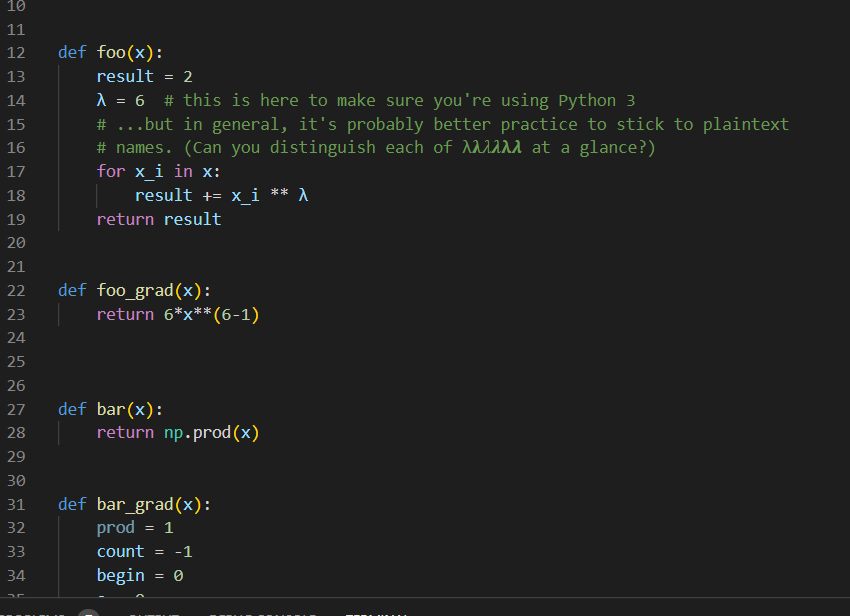
\includegraphics{3_3_1}
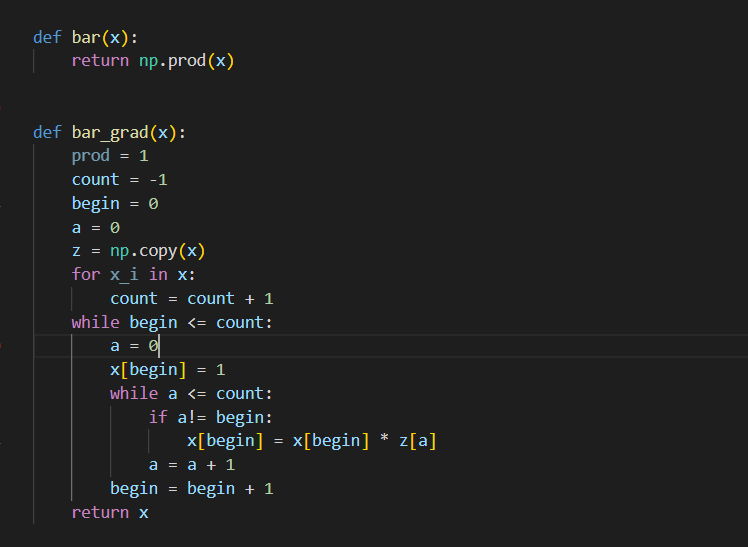
\includegraphics{3_3_2}

\clearpage

\section{Algorithms and Data Structures Review}

For these questions you may find it helpful to review these notes on big-O notation:\\
\url{http://www.cs.ubc.ca/~schmidtm/Courses/Notes/bigO.pdf}

\subsection{Trees}

\blu{Answer the following questions.} You do not need to show your work.
\begin{enumerate}
\item What is the maximum number of \emph{leaves} you could have in a binary tree of depth $l$?
\ans{$2^l$}
\item What is the maximum number of \emph{internal nodes} (excluding leaves) you could have in a binary tree of depth $l$?
\ans{$2^l-1$}
\end{enumerate}
Note: we'll use the standard convention that the leaves are not included in the depth, so a tree with depth $1$ has 3 nodes with 2 leaves.

\clearpage

\subsection{Common Runtimes}

\blu{Answer the following questions using big-$O$ notation.} You do not need to show your work.
\begin{enumerate}
\item What is the cost of running the mergesort algorithm to sort  a list of $n$ numbers?
\ans{$O(nlogn)$}
\item What is the cost of finding the third-largest element of an unsorted list of $n$ numbers?
\ans{$O(n)$}
\item What is the cost of finding the smallest element greater than 0 in a \emph{sorted} list with $n$ numbers?
\ans{$O(n)$}
\item What is the cost of finding the value associated with a key in a hash table with $n$ numbers? \\(Assume the values and keys are both scalars.)
\ans{$O(1)$}
\item What is the cost of computing the matrix-vector product $Ax$ when $A$ is $n \times d$ and $x$ is $d \times 1$?
\ans{$O(nd)$}
\item What is the cost of computing the quadratic form $x^TAx$ when $A$ is $d \times d$ and $x$ is $d \times 1$?
\ans{$O(d^2)$}
\item How does the answer to the previous question change if $A$ has only $z$ non-zeroes? (You can assume $z \geq d$)
\ans{$O(z)$}
\end{enumerate}

\clearpage

\subsection{Running Times of Code}

Your repository contains a file named \texttt{bigO.py}, which defines several functions
that take an integer argument $N$. For each function, \blu{state the running time as a function of $N$, using big-O notation}.
\ans{\\
$func1: O(N)\\
func2: O(N)\\
func3: O(1)\\
func4: O(N^2)$
}

\clearpage

\section{Data Exploration}


  Your repository contains the file \texttt{fluTrends.csv}, which contains estimates
  of the influenza-like illness percentage over 52 weeks on 2005-06 by Google Flu Trends.
  Your \texttt{main.py} loads this data for you and stores it in a pandas DataFrame \texttt{X},
  where each row corresponds to a week and each column
  corresponds to a different
  region. If desired, you can convert from a DataFrame to a raw numpy array with \texttt{X.values()}.

  \subsection{Summary Statistics}

  \blu{Report the following statistics}:
  \begin{enumerate}
  \item The minimum, maximum, mean, median, and mode of all values across the dataset.
  \ans{\\
    minimum: 0.352000 \\
    maximum: 4.862000 \\
    mean: 1.324625 \\
    median: 1.159000\\
    mode: 0.77}
  \item The $5\%$, $25\%$, $50\%$, $75\%$, and $95\%$ quantiles of all values across the dataset.
  \ans{\\
  $5\%$: 0.46495000000000003\\
  $25\%$: 0.718\\
  $50\%$: 1.1589999999999998\\
  $75\%$: 1.81325\\
  $95\%$: 2.624049999999999\\
  }
  \item The names of the regions with the highest and lowest means, and the highest and lowest variances.% \item The pairs of regions with the highest and lowest correlations.
  \ans{\\
    highest means: WtdILI\\
    lowest means: Pac\\
    highest variances: Mtn\\
    lowest variances: Pac
  }
  \end{enumerate}
  In light of the above, \blu{is the mode a reliable estimate of the most ``common" value? Describe another way we could give a meaningful ``mode" measurement for this (continuous) data.} Note: the function \texttt{utils.mode()} will compute the mode value of an array for you.
  \ans{We can choose a small range that contains most values}
  \clearpage

  \subsection{Data Visualization}

  Consider the figure below.

  \centerfig{.9}{visualize-unlabeled.pdf}

  The figure contains the following plots, in a shuffled order:
  \begin{enumerate}
  \item A single histogram showing the distribution of \emph{each} column in $X$.
  \ans{D, because one big column in the graph contains small columns of many color, which also resembles elements in one column. So the big columns in the graph look like distribution of each column in the matrix.}
  \item A histogram showing the distribution of each the values in the matrix $X$.
  \ans{C, each column in the graph cannot be column in the matrix since there is not real separation to differentiate between columns.}
  \item A boxplot grouping data by weeks, showing the distribution across regions for each week.
  \ans{B, because it is a boxplot.}
  \item A plot showing the illness percentages over time.
  \ans{A, because only A and B shows illness percentages over time but B is for the one above.}
  \item A scatterplot between the two regions with highest correlation.
  \ans{F, because dots are almost on the line so the relationship of the two regions is tight}
  \item A scatterplot between the two regions with lowest correlation.
  \ans{E, because the two do not seem to have a tight relationship as Plot F(some dots soar on one side and only increase a little on another)}
  \end{enumerate}

  \blu{Match the plots (labeled A-F) with the descriptions above (labeled 1-6), with an extremely brief (a few words is fine) explanation for each decision.}

  \clearpage
  
  \section{Decision Trees}

  If you run \texttt{python main.py 6}, it will load a dataset containing longitude
  and latitude data for 400 cities in the US, along with a class label indicating
  whether they were a ``red" state or a ``blue" state in the 2012
  election.\footnote{The cities data was sampled from \url{http://simplemaps.com/static/demos/resources/us-cities/cities.csv}. The election information was collected from Wikipedia.}
  Specifically, the first column of the variable $X$ contains the
  longitude and the second variable contains the latitude,
  while the variable $y$ is set to $0$ for blue states and $1$ for red states.
  After it loads the data, it plots the data and then fits two simple
  classifiers: a classifier that always predicts the
  most common label ($0$ in this case) and a decision stump
  that discretizes the features (by rounding to the nearest integer)
  and then finds the best equality-based rule (i.e., check
  if a feature is equal to some value).
  It reports the training error with these two classifiers, then plots the decision areas made by the decision stump.
  The plot is shown below:

  \centerfig{0.7}{q6_decisionBoundary}

  As you can see, it is just checking whether the latitude equals 35 and, if so, predicting red (Republican).
  This is not a very good classifier.

  \subsection{Splitting rule}

  Is there a particular type of features for which it makes sense to use an equality-based splitting rule rather than the threshold-based splits we discussed in class?
  \ans{Yes, for example, feature value 0 map to label value 0 and feature value 1 map to label value 1. This means by knowing whether the feature value equals to 1, we 
  can predict the label (1 if feature=1, else 0)}
  \clearpage

  \subsection{Decision Stump Implementation}

  The file \texttt{decision\string_stump.py} contains the class \texttt{DecisionStumpEquality} which
  finds the best decision stump using the equality rule and then makes predictions using that
  rule. Instead of discretizing the data and using a rule based on testing an equality for
  a single feature, we want to check whether a feature is above or below a threshold and
  split the data accordingly (this is a more sane approach, which we discussed in class).
  \blu{Create a \texttt{DecisionStumpErrorRate} class to do this, and report the updated error you
  obtain by using inequalities instead of discretizing and testing equality.
  Submit your class definition code as a screenshot or using the \texttt{lstlisting} environment.
  Also submit the generated figure of the classification boundary.}

  Hint: you may want to start by copy/pasting the contents \texttt{DecisionStumpEquality} and then make modifications from there.
  \ans{The new error is: 0.253}\\\\
  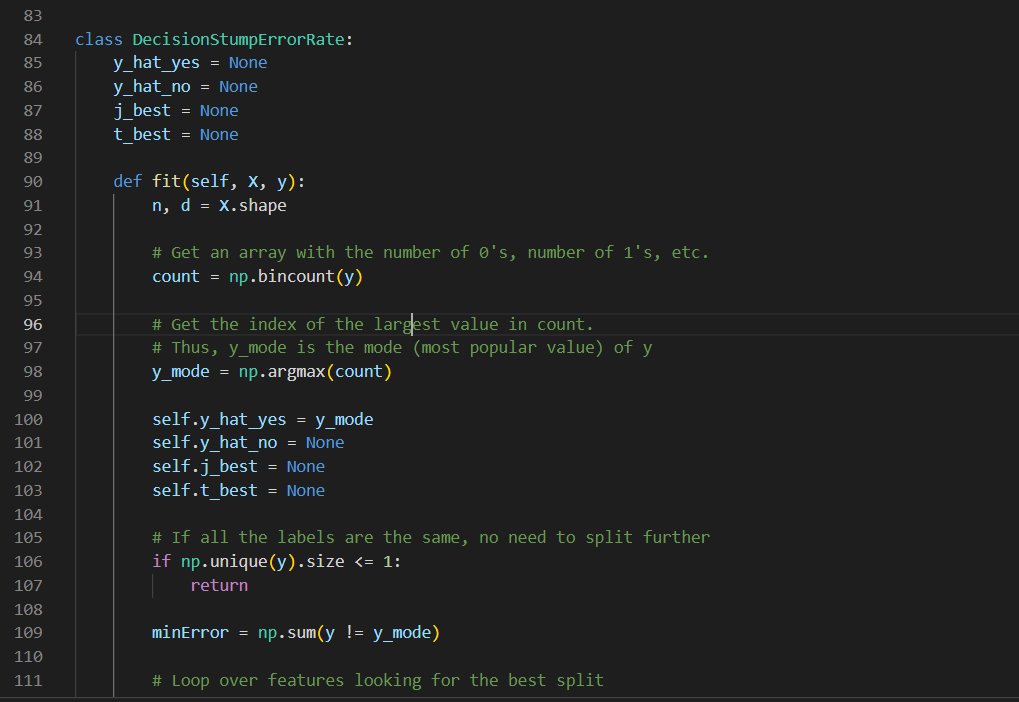
\includegraphics{6_2_1}
  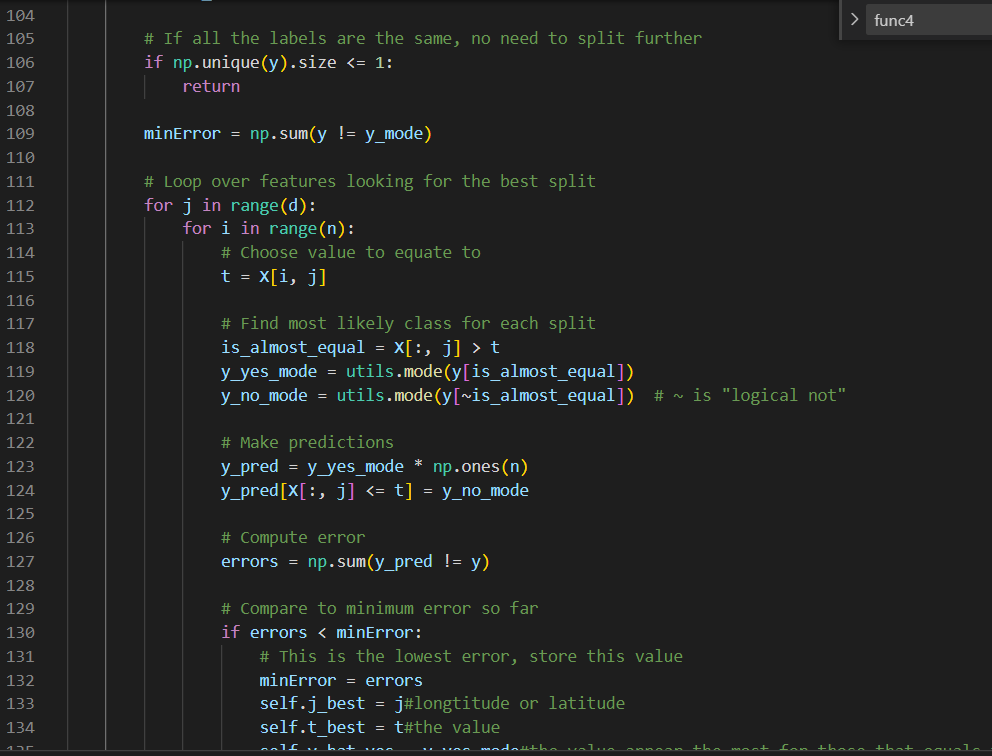
\includegraphics{6_2_2}
  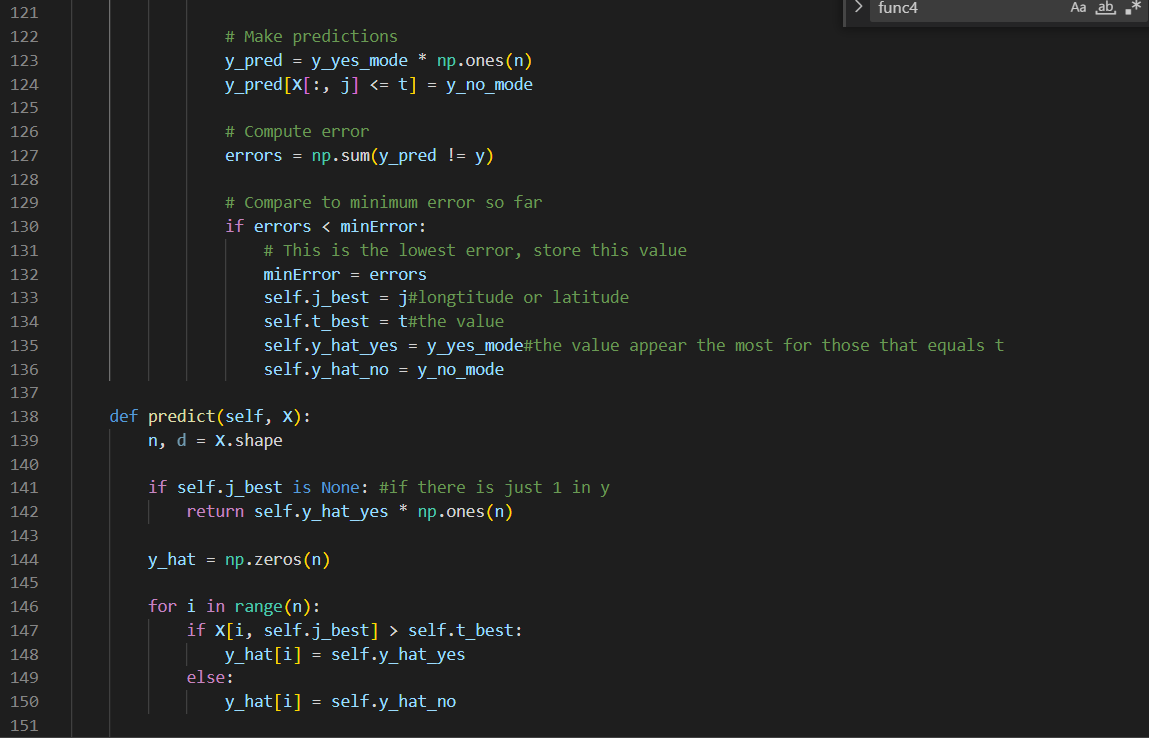
\includegraphics{6_2_3}
  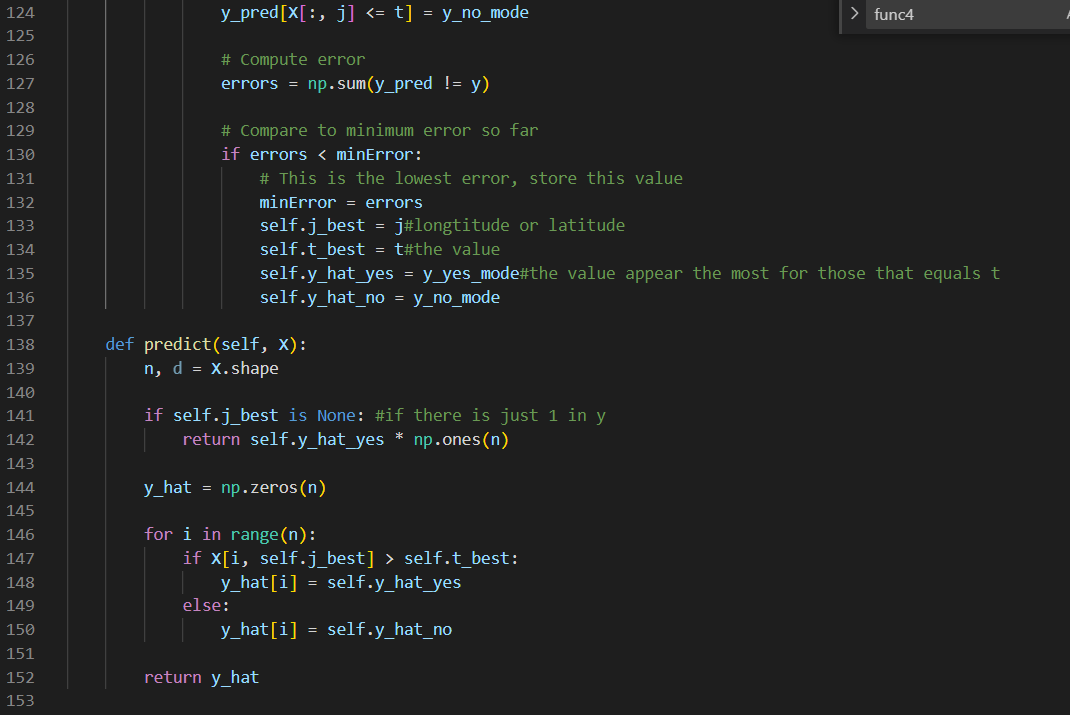
\includegraphics{6_2_4}
  \centerfig{.9}{q6_2_decisionBoundary.pdf}
  \clearpage

  \subsection{Decision Stump Info Gain Implementation}

  In \texttt{decision\string_stump.py}, \blu{create a \texttt{DecisionStumpInfoGain} class that
  fits using the information gain criterion discussed in lecture.
  Report the updated error you obtain.
  Submit your class definition code as a screenshot or using the \texttt{lstlisting} environment.
  Submit the classification boundary figure.}

  Notice how the error rate changed. Are you surprised? If so, hang on until the end of this question!

  Note: even though this data set only has 2 classes (red and blue), your implementation should work
  for any number of classes, just like \texttt{DecisionStumpEquality} and \texttt{DecisionStumpErrorRate}.

  Hint: take a look at the documentation for \texttt{np.bincount}, at \\
  \url{https://docs.scipy.org/doc/numpy/reference/generated/numpy.bincount.html}.
  The \texttt{minlength} argument comes in handy here to deal with a tricky corner case:
  when you consider a split, you might not have any cases of a certain class, like class 1,
  going to one side of the split. Thus, when you call \texttt{np.bincount}, you'll get
  a shorter array by default, which is not what you want. Setting \texttt{minlength} to the
  number of classes solves this problem.
  \ans{The new error is: 0.325}\\\\
  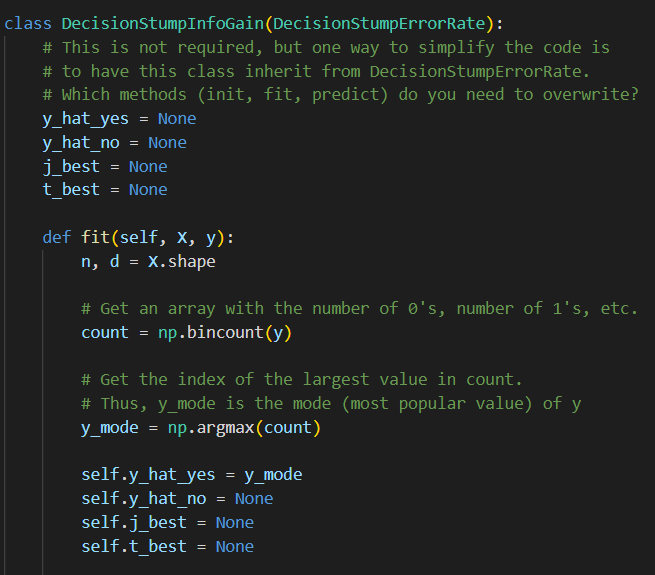
\includegraphics{6_3_1}
  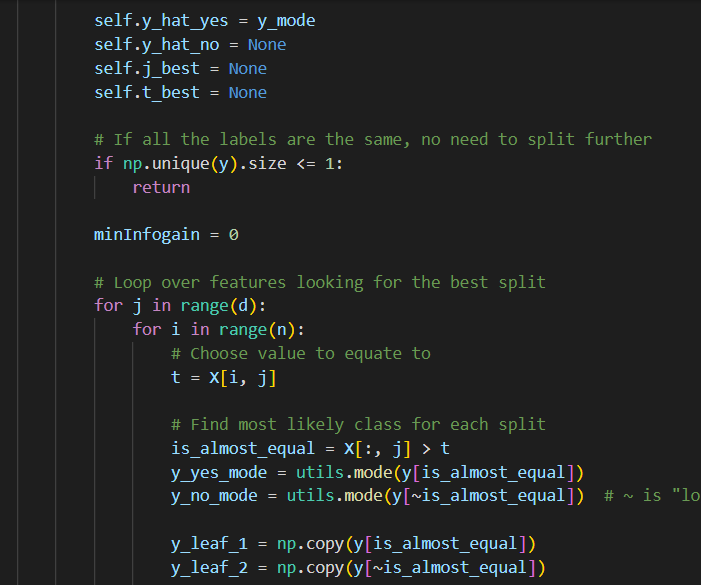
\includegraphics{6_3_2}
  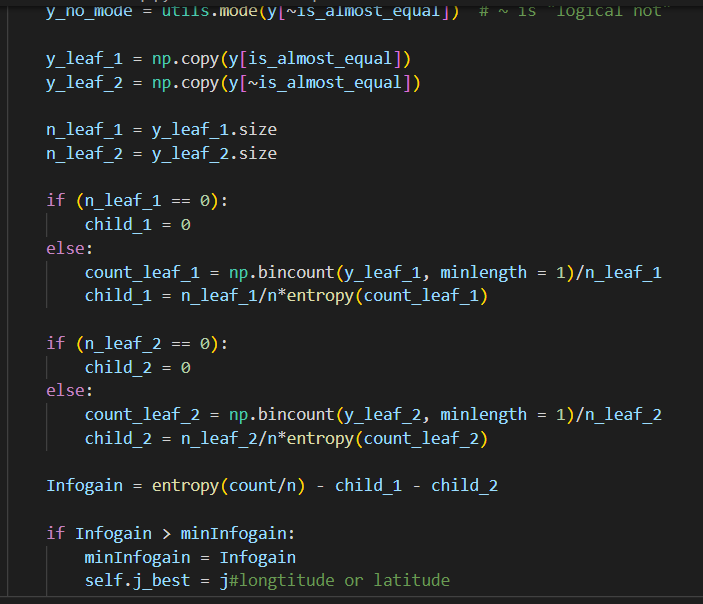
\includegraphics{6_3_3}
  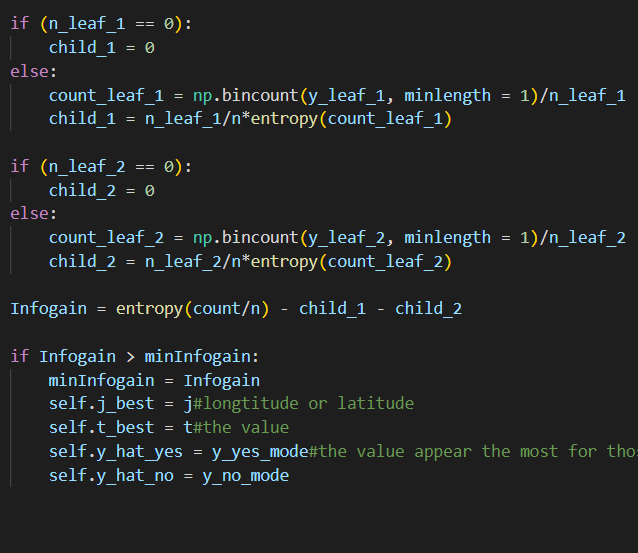
\includegraphics{6_3_4}
  \centerfig{.9}{q6_3_decisionBoundary.pdf}

  \clearpage

  \subsection{Hard-coded Decision Trees}

  Once your \texttt{DecisionStumpInfoGain} class is finished, running \texttt{python main.py 6.4} will fit
  a decision tree of depth~2 to the same dataset (which results in a lower training error).
  Look at how the decision tree is stored and how the (recursive) \texttt{predict} function works.
  \blu{Using the splits from the fitted depth-2 decision tree, write a hard-coded version of the \texttt{predict}
  function that classifies one example using simple if/else statements
  (see the Decision Trees lecture). Submit this code as a plain text, as a screenshot or using the \texttt{lstlisting} environment.}

  Note: this code should implement the specific, fixed decision tree
  which was learned after calling \texttt{fit} on this particular data set. It does not need to be a learnable model.
  You should just hard-code the split values directly into the code.
  Only the \texttt{predict} function is needed.

  Hint: if you plot the decision boundary you can do a quick visual check to see if your code is consistent with the plot.
  \\\\
  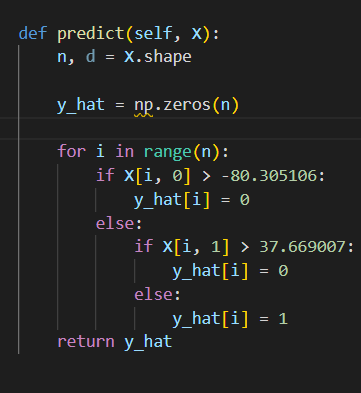
\includegraphics{6_4}
  \clearpage

  \subsection{Decision Tree Training Error}

  Running \texttt{python main.py 6.5} fits decision trees of different depths using the following different implementations:
  \begin{enumerate}
  \item A decision tree using \texttt{DecisionStumpErrorRate}
  \item A decision tree using \texttt{DecisionStumpInfoGain}
  \item The \texttt{DecisionTreeClassifier} from the popular Python ML library \emph{scikit-learn}
  \end{enumerate}

  Run the code and look at the figure.
  \blu{Describe what you observe. Can you explain the results?} Why is approach (1) so disappointing? Also, \blu{submit a classification boundary plot of the model with the lowest training error}.

  Note: we set the \verb|random_state| because sklearn's \texttt{DecisionTreeClassifier} is non-deterministic. This is probably
  because it breaks ties randomly.

  Note: the code also prints out the amount of time spent. You'll notice that sklearn's implementation is substantially faster. This is because
  our implementation is based on the $O(n^2d)$ decision stump learning algorithm and sklearn's implementation presumably uses the faster $O(nd\log n)$
  decision stump learning algorithm that we discussed in lecture.\\
  \ans{Firstly, plot for infogain and sklearn is the same so I think sklearn might be using this approach. Secondly, the error rate approach has better results at small depth
  but at larger depth, sklearn and infogain is better while error rate approach did not improve. I believe this is because error rate approach did not split more after depth 4 so even we increase the maximum depth,
  the approach's tree did not grow and improve the accuracy. This is also the reason that it is disappointing. Thirdly, sklearn and infogain went to 0 at depth 8. However, since the tree is so deep, I think they literally have one object per leaf.}\\

  \centerfig{.9}{q6_5_decisionBoundary.pdf}
  \clearpage

  \subsection{Comparing implementations}

  In the previous section you compared different implementations of a machine learning algorithm. Let's say that two
  approaches produce the exact same curve of classification error rate vs. tree depth. Does this conclusively demonstrate
  that the two implementations are the same? If so, why? If not, what other experiment might you perform to build confidence
  that the implementations are probably equivalent?
  \ans{If its the same on just one data set, I don't think the two implementations are the same. We could try it on more data sets and more corner cases of the problem we are solving.
  If they are still the same, try putting more types of input like images,... since one implementation can deal with a wider range of data type than the other. If they are still have the same results,
  they probably equivalent.}


\vspace{25pt}
\textbf{HAVE YOU DOUBLE CHECKED THAT YOU'RE FOLLOWING ALL THE ASSIGNMENT SUBMISSION INSTRUCTIONS POSTED ON PIAZZA???}

\end{document}